To begin identifying an appropriate development methodology, it is necessary to
understand the project requirements. The project requirements and features are
agreed over a number of meetings with the primary stakeholders. 

At this point, the development methodology can be determined. Since we are
looking for an iterative and incremental development process, Agile Software
Development Methodology will be followed. This also enables a time-boxed iterative approach. Agile methods are focused on different aspects of the software development life cycle. Two of the most well known agile methodologies are Scrum and XP.

Scrum is an agile project management technique that focuses more on the
management of software development projects. The product is completed in a
series of one to four week iterations, or sprints. Before each sprint, a
planning meeting is held to define which features will be implemented during
that sprint. Similarly, XP (Extreme Programming) is an agile methodology which
is designed for small, co-located teams aiming to get quality and productivity
as high as possible. It does this through the use of rich, short, informal
communication paths with emphasis on skill, discipline and understanding at the personal level, minimizing all intermediate work products.

As this is a college project and tight time constraints apply, it is quite
difficult to follow a particular methodology. Scrum focuses on the management
side of the project whereas XP focuses more on the actual programming
practices. It is more preferable if various elements from both methodologies
can be used, since they address different areas and complement each other.

Therefore, it was decided to focus on managing the software project using the scrum
approach and adopt characteristics that suit the project. Weekly meetings are planned to organise the division
of work and for the team to get up to speed with all the tasks in progress and recently
completed. An agenda for each meeting is stored in an online document, that
each team member may add to. 

To encourage a more agile development the online collaboration tool
Trello is used. This tool gives access to a visual board that displays the
ongoing tasks. These tasks are represented as cards with labels and priorities. 
Trello is very similar in concept to the scrum board, as shown in fig 2.

\begin{figure}[here]
\begin{minipage}{\textwidth}  
\begin{center}
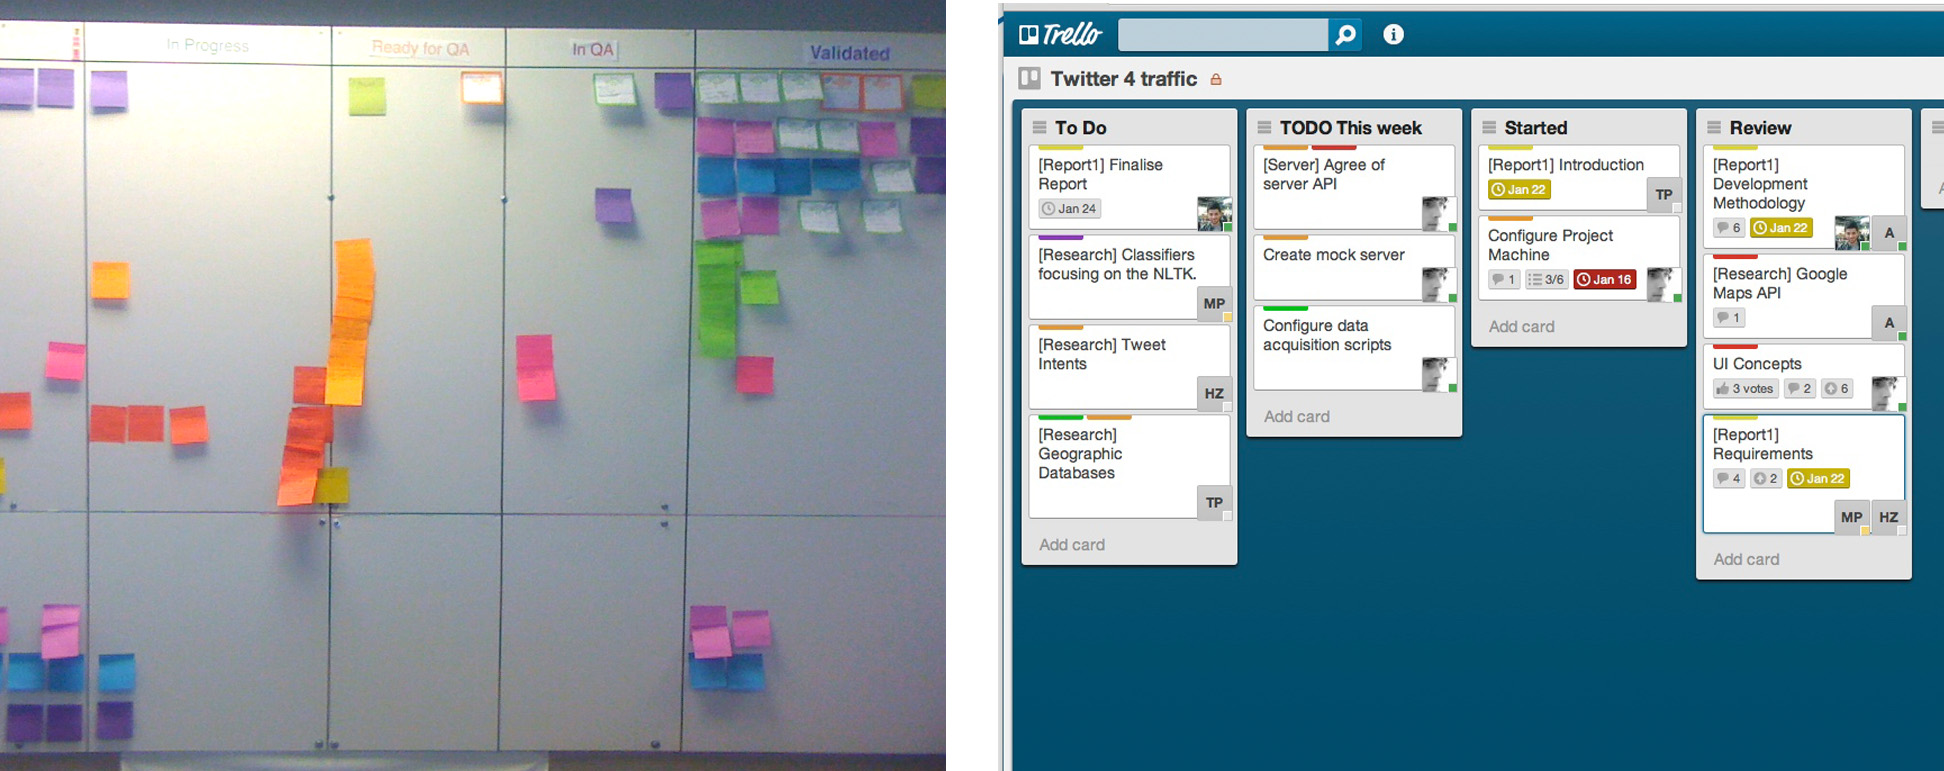
\includegraphics[width=0.95\textwidth]{images/scrumboard.jpg}
\end{center}
\vspace{-20pt}
\caption[Caption for LOF]{Scrum Board and Trello\footnotemark}
\end{minipage} 
\end{figure}
\footnotetext{Left: Drew Stephens \url{flickr.com/photos/dinomite/3695570625}, Right: \copyright \url{Trello.com}}

It was agreed that adopting techniques from XP would help to
improve the development process. Pair programming is one of those techniques the team would strive to adopt.
Two programmers work alongside on the same code and together they develop a single feature. Constant refactoring is another key practice to be adopted. Any
time the two find a section of code that appears hard to understand or overly
complex, they are to revise it, constantly simplifying and improving it. Furthermore, a test driven approach will be taken during this development.
However because of the nature of the project being partly research based and
the results being quite subjective, it is difficult to test effectively. Hence,
the development of the mobile application will be test-driven whereas for the
server development it will not be possible to follow test driven approach so strictly\cite{Cockburn}. These techniques improve the code quality and team focus.

For the division of work amongst the team, more flexibility will be achieved by maximising the use of the members previous experience. A division has been decided where two members of the team will focus on the mobile application, three on the server side and the final person will move between these tasks as necessary. A team leader is also designated with the aim of coordinating the two development efforts.  

To achieve parallel development, the server API will be agreed and mocked-up returning a static data set. That way, those developing the mobile application can work independently from those working on the server.

